\section{Numeryczna reprezentacja liczb rzeczywistych}
%%%%%%%%%%%%%%%%
\begin{frame}{Reprezentacja zmiennoprzecinkowa (float)}
    Należy pamiętać o ułomności reprezentacji zbioru liczb rzeczywistych $\mathbb{R}$ w rzeczywistym świecie skończonych komputerów.
    \begin{block}{}
    $F$ - zbiór liczb zmiennoprzecinkowych (floating-point):\newline
    \begin{columns}
        \column{0.45\linewidth}
            $\beta$ - podstawa,\newline
            $t$ - dokładność,\newline
            $L, U$ - zakres wykładnika\newline
        \column{0.45\linewidth}
            $d_i$ - liczby całkowite,
            $0 \le d_i \le \beta - 1, i=1,...,t$
            $L \le e \le U$
    \end{columns}
    $x \in F$ ma wartość:
    \[
    x = \pm \underbrace{\left(\frac{d_1}{\beta} + \frac{d_2}{\beta^2} + ... + \frac{d_t}{\beta^t}\right)}_\text{mantysa} \cdot \beta^{\overbrace{e}^\text{cecha}}
    = \pm \sum_{i=1}^{t} \frac{d_i}{\beta^i} \cdot \beta^e
    \]        
    System $F$ jest {\it unormowany}, gdy $\forall_{x \ne 0} d_i \ne 0$.
    \end{block}

\end{frame}
%%%%%%%%%%%%%%%%
\begin{frame}{Reprezentacja zmiennoprzecinkowa (float)}
    W komputerze jest przechowywana liczba całkowita $\beta^t \cdot m$ (zgodnie z wybranym systemem kodowania).

    $\beta^{1-t}$ - oszacowanie względnej dokładności arytmetyki

    \hspace{0.5cm}
    \centering
    \begin{tabular}{| l | c | c | c | c | c |}
    \hline
    Komputer & $\beta$ & $t$ & $L$ & $U$ & $\beta^{1-t}$ \\ \hline
    CDC CYBER 72 		& 2  & 48 & -975 	& 1070 & $7.11 \cdot 10^{-15}$ \\ \hline
    Cray-1 				& 2  & 48 & -16384	& 8191 & $7.11 \cdot 10^{-15}$ \\ \hline
    IBM 360, 370 		& 16 & 6  & -64		& 63   & $9.54 \cdot 10^{-7}$ \\ \hline
    IBM 360, 370 (DP) 	& 16 & 14 & -64 	& 63   & $2.22 \cdot 10^{-16}$ \\ \hline
    IBM PC XT / AT 		& & & & & \\ \hline
    Delta (VAX) 		& & & & & \\ \hline
    \end{tabular}
\end{frame}
%%%%%%%%%%%%%%%%
\begin{frame}{Reprezentacja zmiennoprzecinkowa (float)}
    \begin{block}{Ważne}
    $F$ nie jest kontinuum - więcej - jest skończony o liczbie elementów wyrażonych wzorem:
    \[
    2 \cdot \left(\beta - 1 \right) \cdot \beta^{t-1} \cdot \left( U - L + 1 \right) + 1
    \]
    \begin{flushright}
        {\it Zadanie:} sprawdzić
    \end{flushright}
    \end{block}
\end{frame}
%%%%%%%%%%%%%%%%
\begin{frame}{Reprezentacja zmiennoprzecinkowa (float)}
    Elementy $F$ nie są równomiernie rozłożone na osi:
    $\beta = 2, t = 3, L = -1, U = 2$ \hspace{5mm} (33 elementy):
    \begin{center}
    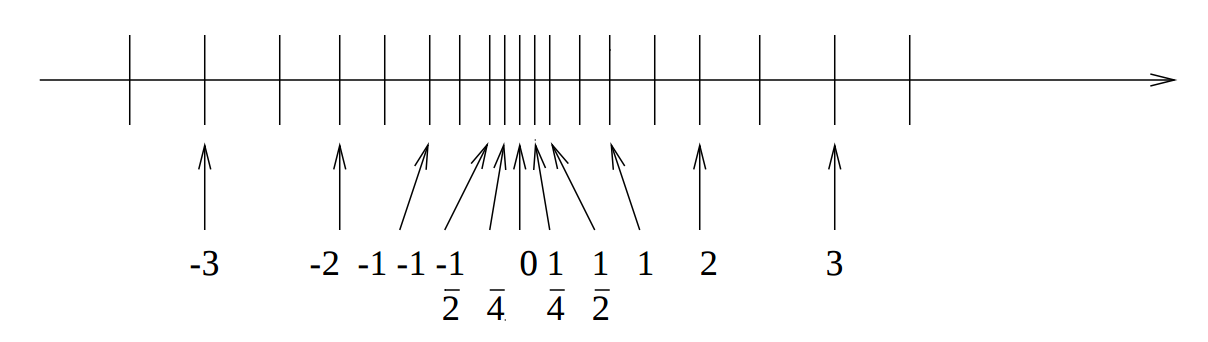
\includegraphics[width=0.8\linewidth]{img/2/2_1_axis}
    \end{center}

    Każdy element $F$ reprezentuje cały przedział liczb $\mathbb{R}$\newline 
    $x$ - l. rzeczywista $\in$ zakresu $F$,\newline
    $fl(x)$ - reprezentacja zmiennoprzecinkowa liczby $x$

    \[
    \left| \frac{fl(x) - x}{x} \right| \le \frac{1}{2} \beta^{1-t}
    \]

    \begin{flushright}
        {\it Zadanie:} sprawdzić
    \end{flushright}
\end{frame}
%%%%%%%%%%%%%%%%
\begin{frame}{Reprezentacja zmiennoprzecinkowa (float)}
    \begin{alertblock}{Uwaga}
        $0.1$ - często krok w algorytmach\newline
        Czy 10 kroków o długości $0.1$ to to samo co 1 krok = $1.0$?\newline
        W systemie o $\beta = 2^n$ - {\bf nie!}
        \[
        0.1_{10} = 0.0(0011)_2 = 0.0(12)_4 = 0.0(6314)_8 = 0.199999..._{16}
        \]

        Reprezentacja $0.1$ urywa się o $t$ cyfrach. Dodanie 10 tak uzyskanych liczb nie da dokładnie $1.0$.
    \end{alertblock}
\end{frame}
%%%%%%%%%%%%%%%%
\subsection{Dokładność reprezentacji zmiennoprzecinkowej}
\begin{frame}{Reprezentacja zmiennoprzecinkowa (float)}
    \[
    x = s \cdot 2^c \cdot m
    \]\[
    m = \sum_{i=1}^{\infty} e_i \cdot 2^{-i}
    \]\[
    e_i = \left\{ 
              \begin{array}{ll}
                  0 \\
                  1
              \end{array}
        \right.
    \]

    \begin{block}{Reprezentacja mantysy}
        Mantysa jest reprezentowana jako:
        \[
        m_t = \sum_{i=1}^{t}e_i \cdot 2^{-i} + \underbrace{e_{t+1} \cdot 2^{-t}}_\text{zaokrąglenie}
        \]
    \end{block}
\end{frame}
%%%%%%%%%%%%%%%%
\begin{frame}{Reprezentacja zmiennoprzecinkowa (float)}
    a)\newline

    \centering
    \begin{tabular}{|*{5}{p{.75cm}|}}
        \hline
        t & t+1 & t+2 & ... &  \\ \hline
          & 0   & 1   & ... & 1 \\ \hline
    \end{tabular}
    \[
    m = \underbrace{\sum_{i=1}^{t} e_i \cdot 2^{-i} + 0 \cdot 2^{-(t+1)}}_{m_t} +
        \underbrace{\sum_{i=t+2}^{\infty} 1 \cdot 2^{-i}}_{
            \frac{1}{2^{t+1}} = 2^{-(t+1)}
        }
    \] \[
    m - m_t = 2^{-(t+1)}
    \]
\end{frame}
%%%%%%%%%%%%%%%%
\begin{frame}{Reprezentacja zmiennoprzecinkowa (float)}
    b)\newline

    \centering
    \begin{tabular}{|*{5}{p{.75cm}|}}
        \hline
        t & t+1 & t+2 & ... &  \\ \hline
          & 1   & 0   & ... & 0 \\ \hline
    \end{tabular}
    \[
    m = \sum_{i=1}^{t} e_i \cdot 2^{-i} + 2^{-(t+1)}
    \]\[
    m_t = \sum_{i=1}^{t} e_i \cdot 2^{-i} + 2^{-t}
    \] \[
    m_t - m = 2^{-(t+1)} \left| \frac{m - m_t}{m} \right| \le \frac{2^{-(t+1)}}{1/2} = 2^{-t}
    \]
\end{frame}

%%%%%%%%%%%%%%%%